\documentclass[a4paper,12pt,titlepage]{article}
\usepackage[T1]{fontenc}
\usepackage[brazilian]{babel}
\usepackage{enumerate}
% setspace - \doublespace
% fullpage - ??
\usepackage{verbatim,url}
\usepackage{graphicx}
\usepackage{amsmath, amssymb}
\usepackage[numbers,sort&compress]{natbib}
%\usepackage[numbers]{natbib}
\usepackage{fullpage,setspace}
\usepackage{ae}
\usepackage[utf8]{inputenc}

\newenvironment{changemargin}[2]{\begin{list}{}{
   \setlength{\topsep}{0pt}\setlength{\leftmargin}{0pt}
   \setlength{\rightmargin}{0pt}
   \setlength{\listparindent}{\parindent}
   \setlength{\itemindent}{\parindent}
   \setlength{\parsep}{0pt plus 1pt}
   \addtolength{\leftmargin}{#1}\addtolength{\rightmargin}{#2}
}\item }{\end{list}}

\doublespace
\begin{document}

\pagestyle{empty}
\begin{center}
\large \bf Universidade de São Paulo\\[-0.5cm]
Instituto de Física de São Carlos\\[4.5cm]
\end{center}

{\LARGE O pensamento ideal\\[0.5cm] 
%  \noindent\normalsize \centerline{\bf (projeto de pesquisa)} \\[.3cm]}\\[1.5cm]
}
\vfill 
%\begin{flushright}
%\large
%  {\bf Candidato:} Renato Fabbri$\quad\quad\quad\quad\quad\quad\quad\quad\quad\quad\quad\quad\quad$\\
%  {\bf Orientador proposto:} Prof. Dr. Osvaldo Novais de Oliveira Junior\\
%%  {\bf Co-Orientador:} Prof. Dr. Luciano da Fontoura Costa\\
%\end{flushright}
\vspace{5mm}
\begin{center}
\large
    dezembro de 2012
\end{center}


\newpage
\thispagestyle{empty}
\mbox{}

\begin{abstract}
O pensamento é constituido de ideias. Estas são passíveis de uma
modelagem bastante genérica, em que qualquer conjunto de ideias é uma ideia.
Uma forma padrão é convencionada
para o espaço de ideias e um mecanismo de \emph{bootstrap}, serve de base para
análises sobre a estrutura da rede em si. A geração de novas ideias apresenta
modificações relevantes na topologia. Este trabalho se propõe a obter uma
descrição física e formal do pensamento.
\end{abstract}

\newpage

\newpage
\thispagestyle{empty}
\mbox{}
\newpage
\thispagestyle{empty}
\mbox{}


\pagestyle{plain}
\tableofcontents
\newpage

\newpage
\thispagestyle{empty}
\mbox{}

\newpage
\thispagestyle{empty}
\mbox{}

\section{Introdução}
Do pensamento. Deleuze e Derrida com a expansão dimensional do signo:
todo significado nada mais é do que um conjunto específico de significantes
de outros signos.
%\begin{figure}[h!]
%    \begin{center}
%        \includegraphics[scale=.3]{figuras/rederf_.png}
%        \caption{Rede do \emph{facebook} do candidato.
%        1-amigos da igreja da esposa, 2-amigos da graduação e relacionados, 3-família por parte de pai e mãe,
%        4-conhecidos do {\bf IFSC}, 5-conhecidos através do trabalho engajado em tecnologias sociais. Em 'a' está
%        a esposa do candidato, e em 'b' o irmão.}
%        \label{fig:face}
%    \end{center}
%\end{figure}


\section{Teoria física do pensamento}
\subsection{Descrição de uma ideia}
No espaço ideal de ideias, qualquer conjunto conectado
de ideias é uma ideia.

\begin{figure}[h!]
    \begin{center}
        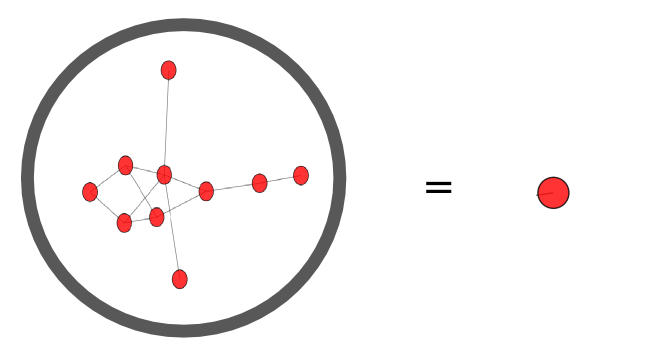
\includegraphics[scale=.3]{figs/variasUma.png}
        \caption{Qualquer conjunto de ideias é uma ideia}
        \label{fig:face}
    \end{center}
\end{figure}


Uma ideia ideal é aquela que possui infinitas representações
com cada número de ideias.

\begin{figure}[h!]
    \begin{center}
        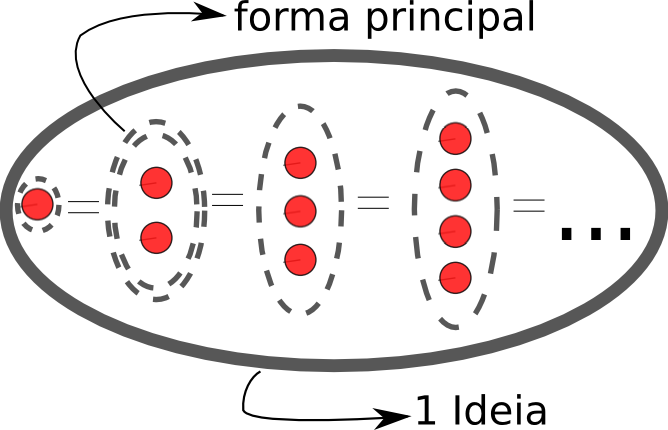
\includegraphics[scale=.3]{figs/ideia2.png}
        \caption{Uma ideia ideial com infinitas representações para cada número de ideias. A forma
        principal desta ideia tem 2 ideias.}
        \label{fig:face}
    \end{center}
\end{figure}


A forma principal de uma ideia é a representação mais ocorrente, preferencial.
É uma referência à ideia. As outras formas são equivalentes e também podem ocorrer.

As ideias com a forma principal de cardinalidade 1 (número de ideias internas)
são as mais ocorrentes. Nos testes
abaixo, mais de 90\% das ideias possuem forma principal com cardinalidade 1,
menos de 5\% possuem cardinalidade maior que 2.
A ideias com formas principais com mais elementos são consideradas
típicas de processos de aprendizado ou de objeto de foco, como em pesquisa.

\subsection{Espaço de ideias}
Em um espaço ideal de ideias, todas ideia é ideal. Dispostas
na forma padrão, as representações de mesma cardinalidade
formam um plano de cardinalidade. Uma representação em um plano
de cardinalidade $x$ é uma conexão entre $x$ ideias. As conexões
de uma ideia em sua forma principal feita entre as formas principais das ideias que a compõe é sua
incidência.

\begin{figure}[h!]
    \begin{center}
        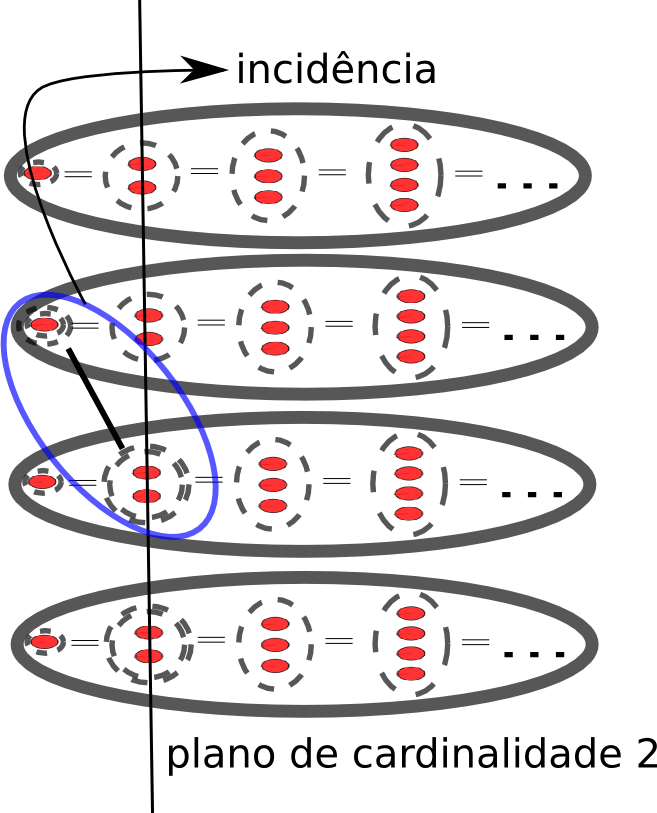
\includegraphics[scale=.3]{figs/planoIdeias}
        \caption{Uma ideia ideial com infinitas representações para cada número de ideias. A forma
        principal desta ideia tem 2 ideias.}
        \label{fig:face}
    \end{center}
\end{figure}


% FIGURA da forma padrão




\subsection{Bootstrap}
3000 ideias com formas principais de cardinalidade 1. São adicionadas 5\% de ideias
cuja forma principal tem cardinalidade 2, 0.2\% de ideias com forma principal de cardinalidade 3 e 0.1\% com 4.
Estas ideias com cardinalidade 2, 3 e 4 são feitas a partir das de cardinalidade 1. Podem também
estar presentes nas composições umas das outras.

Este bootstrap tem o propósito de simular um contexto de pensamento, um 'episódio focado'.

Assim, os seguintes testes foram feitos para validar com métricas o espaço:

\begin{enumerate}
    \item Todas as ideias de formas principais 2,3 e 4 são formadas a partir de ideias de forma principal com cardinalidade 1.
    \item As ideias cuja forma principal tem cardinalidade 2 ou 3 são possuem em sua composição ideias cuja forma principal possuem cardinalidade 2 ou 3
    \item Em uma ideia cuja forma principal tem cardinalidade 2, uma ideia de FP com cardinalidade 3 faz parte de sua composição. Desta, uma ideia com FP de cardinalidade 4 faz parte.
    \item As ideias de cardinalidades 2, 3 e 4 são altamente conectadas.
\end{enumerate}

\begin{figure}[h!]
    \begin{center}
        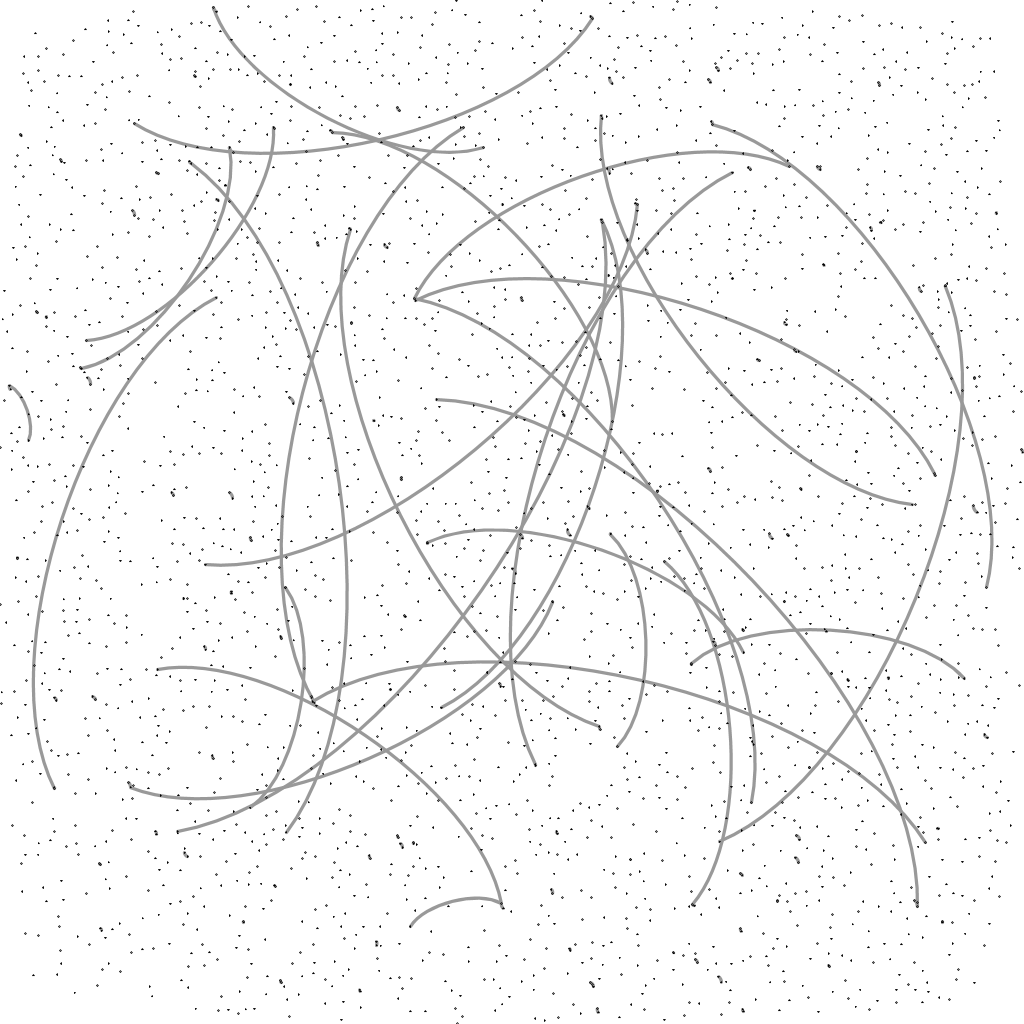
\includegraphics[scale=.3]{figs/boot1}
        \caption{Rede de ideias resultante do \emph{bootstrap}.}
        \label{fig:boot}
    \end{center}
\end{figure}

\subsection{Formação de novas ideias}
A ideação $\Gamma$ é considerada como uma ideia primeira, ela contém todas as N ideias $\{\gamma_i\}_0^{N}$ relacionadas ou apenas destacadas em um pensamento.
A rede cognitiva se encontra em uma representação de alta ordem da ideação. Ou seja, todas as ideias de uma ideação estão conectadas por um click abstrato de alta ordem.

As ideias $\gamma_i$ podem se conectar em um processo ``top-down'', com a divisão de ideias importantes em 2 ou 3 partes tipicamente, ou ``bottom-up'', com a conexão das ideias $\gamma_i$ em grupos de 2 ou 3 partes tipicamente. 4 ou mais ideias tendem fortemente a se subdividirem em grupos de 2 e 3, portando grupos maiores de ideias podem ser desprezados ou restritos aos primos como estruturas cíclicas ou cliques. A divisão em 3 pode ser entendida como mais cara pois destaca e conecta mais ideias do que a divisão em 2. Pode-se entender que a divisão em 3 tende a acrescentar paisagem ao pensamento, ao passo que a divisão em 2 tente a acrescentar mais profundidade ao encadeamento de ideias. Além disso, o 2 pode ser associado à percepção (figura/fundo, claro/escuro, etc) enquanto a divisão ternária é tipicamente ligada ao pensamento mais abstrato.

São consideradas $\kappa_b$ iterações ``bottom-up'' e $\kappa_t$ iterações ``top-down'' de geração de links. Em cada interação, as ideias são conectadas com base em suas importâncias. Assim, a cada iteração de $\kappa_b$ conecta-se mais ideias importantes; a cada iteração de $\kappa_t$ conecta-se ideias obtidas na decomposição de uma ideia importante. As propabilidades de haver divisão em 2 e 3 (top-down) ou aglomeração em 2 e 3 (bottom-up) podem ser consideradas distintas ($p_d(3), p_d(2), p_a(3), p_a(2)$ com $p_d(2)+p_d(3)=1$ e  $p_a(2)+p_a(3)=1$). Pode haver condicional com relação às formações que já ocorreram ou da qual a ideia faça parte.

Uma alternativa é estabelecer um número máximo de links criados. Algum tipo de limiar de custo para o pensamento pode facilitar um critério de parada mais elaborado. 

\subsection{Atribuição de importância}
A atribuição de importância às ideias pode ser fixa ou variar com relação
à conectividade ou outras medidas de centralidade.
A cardinalidade da forma principal da ideia pode também contribuir para sua importância
pois esta deve ser crucial para o problema sendo atacado, já que a elevada cardinalidade tem custo.


\subsubsection{Top-down}
Com uma roleta sobre as X ideias mais importantes ou acima de um limiar, é escolhida a ideia. Esta ideia é explorada em sua forma principal com maior chance, mas não obrigatoriamente. Pode-se considerar que haverá somente formas principais com 2 ou 3 ideias; pode-se também considerar que haverá 4 ou mais ideias com chance muito menor, e somente como ciclos ou cliques.

\subsubsection{Bottom-up}
Com um 'limiar de volição', despreza-se todas as importâncias abaixo deste limiar. Então
uma roleta escolhe qual ideia dispara a nova ideia. A probabilidade
de cada ideia disparar a nova ideia é;
\begin{equation}
\frac{p_k}{\sum_ip_i}\;\;,\;\; \forall \;p_k,p_i > limiar
\end{equation}

Então, uma nova roleta escolhe a ideia com a qual a primeira
se conectou. A probabilidade de cada ideia ser escolhida é:
\begin{equation}\label{eq:ideiaAdd}
\frac{p_i}{\sum_jp_j}\;\;,\;\; \forall \;p_i,p_j > limiar\;,\; p_i,p_j \;\neq\; p_k
\end{equation}

Depois desta etapa, a ideia pode continuar crescendo. Então é feito um novo teste, com base nas
probabilidades das ideias já selecionadas. Pode-se considerar que a probabilidade
da ideia possuir ainda uma terceira ideia é:

\begin{equation}\label{eq:ideiaCresce}
\alpha\frac{p_k+p_i}{\sum_jp_j}
\end{equation}

Com $\alpha$ dependente do contexto e personalidade. A adição de mais ideias
pode ser feita com a aplicação sucessiva das equações~\ref{eq:ideiaAdd} e~\ref{eq:ideiaCresce},
variando $\alpha$.

\subsection{Caracterização da rede com as ideias formadas}
Para cada uma das 1-4 formações de redes do \emph{bootstrap}, são geradas
1-5 ideias novas e acompanhadas as características da rede através de medidas e visualizações.



\subsection{Variações de importância}
A importância das ideias podem sofrer modificações, alterando as propriedades
das ideias geradas. A princípio, distinguimos entre soma direta de importância em todas
as ideias (ou \emph{bias}) e soma aleatória de importância. O primeiro pode ser associado
à religiosidade, hipomania e esimulação. O segundo pode ser associado ao fanatismo,
epifanias e episódios traumáticos.

A geração de ideias sucessivas permite um acompanhamento da importância distribuida
entre as ideias. Após o bootstrap, são adicionadas ideias até a convergência da topologia
e analisada a rede resultante.

\subsection{Motivos de formação de ideias e formações patológicas}
Exemplos de motivos ou formações patológicas:
\begin{itemize}
    \item Só forma ideia com 4 ideias internas como forma principal.
    \item Só forma ideias disparadas pela segunda ideia mais importante.
    \item Só apresenta ideias cujas formas principais possuem cardinalidade baixa. (depressão ou perda cognitiva)
    \item Só apresenta ideias com importância baixa. (pessoa do contra)
\end{itemize}

\subsection{Caracterização e consequências}
Medidas do bootstrap, medidas da rede antes e depois de novas ideias, medidas da rede depois
de ter ideias até convergirem as medidas. 

A formação das redes a partir de textos, em que cada palavra é associada a uma ideia, pode ser usada para algum tipo de observação empírica.

O que mais?

\clearpage 
\begin{thebibliography}{1}
% Redes complexas 
\bibitem{ldfrc} L. F. Costa; F. A. Rodrigues; G. Travieso; P. R. V. Boas ``Characterization of complex networks: A survey of measurements'', Arxiv preprint cond-mat/0505185, 2005.


\bibitem{fabbriENFMC} 
Fabbri, R. ; Amancio, D. R. ; da F. Costa, Luciano ; Oliveira Junior, O. N., ``Use of complex networks for the analysis of speech.'',XXXIII Encontro Nacional de Física da Matéria Condensadas. Águas de Lindóia / SP. 2010.

\bibitem{fabbriSIFISC} Fabbri, Renato. Costa, Luciano da Fontoura. Oliveira Junior, Osvaldo Novais de. ``Redes complexas no processo de fala.'' Workshop da Pós-Graduação do IFSC. Livro de Resumos, São Carlos : Universidade de São Paulo - USP, Instituto de Física de São Carlos - IFSC, 2010.

\bibitem{scalefree} A.-L. Barabási e R. Albert, ``Emergence of scaling in random networks'', Science, v. 286, p. 509-512, 1997.

\bibitem{fabbriAmancio} Amancio, D. R. ; Fabbri, R. ; Oliveira Jr., O. N. ; Nunes, M.G.V. ; Costa, L. F. , ``Opinion Discrimination Using Complex Network Features. '', 2nd Workshop on Complex Networks, Rio de Janeiro,  2nd Workshop on Complex Networks, 2011.
\bibitem{fabbriVieira} Vieira, V. ; FABBRI, R. ; Travieso, Gonzalo; Oliveira Jr., O. N. ; Costa, L. F. , ``A quantitative approach to evolution of
music and philosophy'', {\bf J. Stat. Mech.} P08010 (2012) 

\bibitem{fabbriACL} Amancio, D. R. ; FABBRI, R. ; Nunes, M. G. V. ; Oliveira Jr., O. N. ; Costa, L. F, ``Distinguishing between Positive and Negative Opinions with Complex Network Features'', TextGraphs-5 - 2010 Workshop on Graph-based Methods for Natural Language Processing - {\bf ACL, Uppsala,} 2010.
% PLN por Redes complexas
\bibitem{whatname} L. da F. Costa, ``What's in a name?'', cond-mat/0309266, Sept. 2003.

\bibitem{textquali} L. Antiqueira, M. das Graças V. Nunes, O.N. Oliveira, L. da F. Costa, ``Strong correlations between text quality and complex networks features'', Physica A, Volume 373, p. 811-820, 2005, URL: (http://arxiv.org/abs/physics/0504033).

\bibitem{summa} L. Antiqueira; O. N. Oliveira; L. F. Costa; M. G. V. Nunes, ``A complex network approach to text summarization'', Information Sciences, v. 179, n. 5, p. 584-599, Elsevier, 2009.

\bibitem{auth} L. Antiqueira; T. A. S. Pardo; M. G. V. Nunes; O. N. Oliveira JR., ``Some issues on complex networks for author characterization'', Inteligencia Artificial (Mexico), p. 1-8, 2007.

% Reconhecimento de emoções pela acústica

\bibitem{nltk} S. Bird; E. Klein; E. Loper, ``Natural language processing with Python'', Oreilly \& Associates Inc, 2009.

\bibitem{aux} S. M. A. Caldeira e O. N. Oliveira Jr., ``Proposta de um ambiente para auxiliar na produção de textos científicos em inglês'', Congresso Nacional de Informática, São Paulo, p. 24, 1991.

\bibitem{regra} R. Hasegawa; R. T. Martins; M. G. V. Nunes, ``ReGra 2002: Caracter{\'\i}sticas e Desempenho``, Relat{\'o}rio T{\'e}cnico NILC-TR-02-8 ICMC-USP, p. 02-08, 2002.

\bibitem{dicion} L. Antiqueira; M. F. Fossey; T. Pedrolongo; J. G. Greghi; R. T. Martins; M. G. V. Nunes, ``A construção do corpus e dos dicionários Inglês-UNL e UNL-português para o projeto EPT-Web'', Série de Relatórios do Núcleo Interinstitucional de Lingüística Computacional NILC - NILC-TR-02-24, Dezembro 2002.

\bibitem{sintat} H. M. Caseli e M. G. V. Nunes, ``Anali: uma ferramenta de análise morfossintática.'', Série de Relatórios do ICMC, 285 (NILC-TR-06-09), Outubro 2006.

\bibitem{thesau} E. G. Maziero; T. A. S. Pardo, ``Interface de Acesso ao TeP 2.0 - Thesaurus para o português do Brasil.'' Série de Relatórios NILC. NILC-TR-08-07, Junho 2008. 

% Reconhecimento de Padrões, ao menos o livro do Prof. Luciano

\bibitem{livro} L. da F. Costa and R. M. Cesar Jr, ``Shape Classification and Analysis: Theory and Practice'', CRC, 2009.

\end{thebibliography}

\end{document}

